% SnapTag, doi:10.1145/2676702.2676719, pp.139–140.
% Source-grounded belongings scenario: Tag, Recall, optional Find.
% Shape cues replace colour cues for this monochrome conceptual illustration.
% No measured efficacy, real-time tracking or exact app-screen reconstruction.
\documentclass[tikz,border=0pt]{standalone}
\usepackage[T1]{fontenc}
\usepackage{helvet}
\renewcommand\familydefault{\sfdefault}
\usepackage{graphicx}
\graphicspath{{../../.local/figures/plots/}}
\usetikzlibrary{arrows.meta}
\tikzset{every node/.style={font=\fontsize{9}{10.5}\selectfont,
  text=black,align=center,inner sep=0pt},
  flow/.style={draw=black,line width=.8pt,
    -{Stealth[length=1.5mm,width=1.2mm]}},
  glyph/.style={draw=black,line width=.8pt,fill=white}}
% Stable associations in every scene and screen: circle=keys, triangle=glasses.
\newcommand{\keycue}[3]{\draw[glyph] (#1,#2) circle (#3);}
\newcommand{\glasscue}[3]{
 \draw[glyph] (#1,#2-#3)--(#1+#3,#2+#3)--(#1-#3,#2+#3)--cycle;}
\newcommand{\glasses}[2]{
 \begin{scope}[shift={(#1,#2)}]
  \draw[black,line width=.8pt] (-32,0) ellipse (22 and 17);
  \draw[black,line width=.8pt] (32,0) ellipse (22 and 17);
  \draw[black,line width=.8pt] (-10,-2) .. controls (-5,-10) and (5,-10) .. (10,-2);
  \draw[black,line width=.8pt] (-54,-5)--(-63,-12) (54,-5)--(63,-12);
 \end{scope}}
\begin{document}
\begin{tikzpicture}[x=1mm,y=1mm,line width=.7pt]
\path[use as bounding box] (0,0) rectangle (240,180);
\draw (8,62) rectangle (232,174);
\node[anchor=west,fill=white,inner sep=1pt] at (12,177) {A. Belongings: trigger situated recall before revealing an answer};
\begin{scope}[shift={(25,174)},x=.095mm,y=-.095mm]


\node[anchor=north west] at (0,90)
 {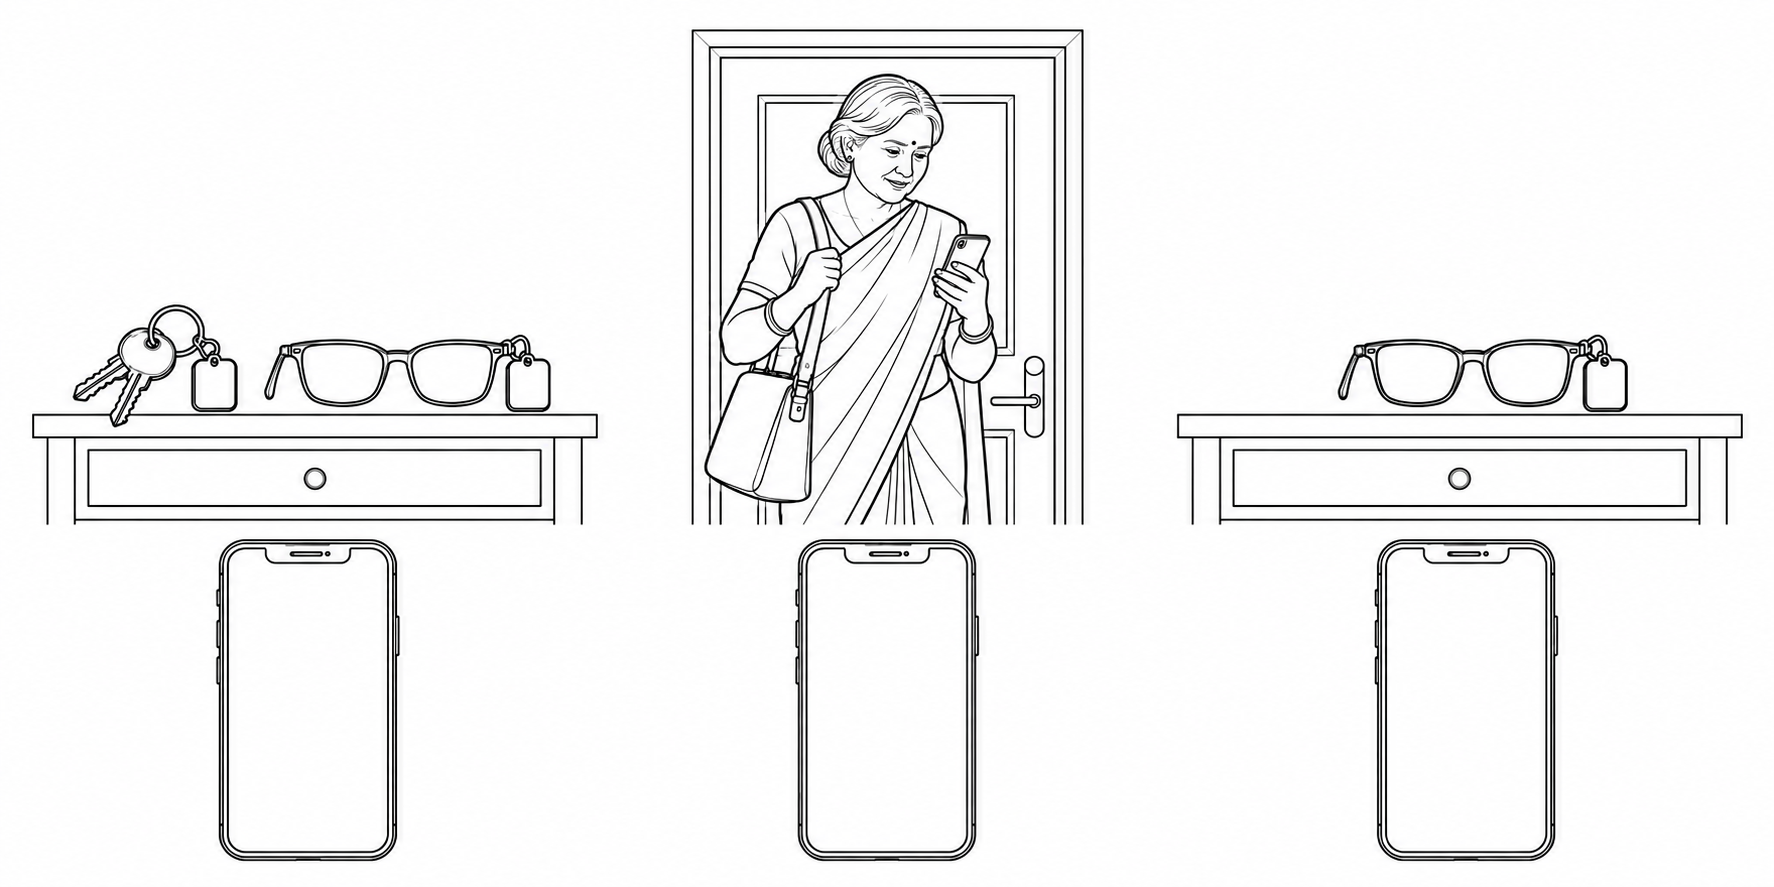
\includegraphics[width=190mm]{artwork-veena.png}};

% Stage labels use the same 9 pt size as all interface text and captions.
\node at (347,45) {Tag objects};
\node at (1000,45) {Veena, 62: recall before leaving};
\node at (1658,45) {Find if needed};
\node at (347,1130) {Near-field communication tags\\mapped to doorway};
\node at (1000,1130) {Prompt\\recollection};
\node at (1658,1130) {Optional identification\\and camera aid};

% Two physical cue identities, preserved in the later contextual prompt.
\keycue{241}{524}{10}
\glasscue{595}{524}{10}
\glasscue{1812}{524}{10}

% Registration: associate object cues with the doorway context.
\node at (347,770) {Doorway};
\keycue{285}{840}{14}
\node[anchor=west] at (315,840) {Keys};
\glasscue{285}{905}{14}
\node[anchor=west] at (315,905) {Glasses};
\node at (347,990) {Associate};

% Recall: show contextual cues without immediately naming the objects.
\node at (1000,770) {Before\\you go};
\keycue{960}{870}{18}
\glasscue{1040}{870}{18}
\node at (1000,975) {Think back};

% Optional fallback: tap to reveal identity; camera aid is a further option.
\node at (1658,770) {Tap to\\reveal};
\glasscue{1658}{842}{16}
\glasses{1658}{905}
\node at (1658,955) {Glasses};
\draw[black,line width=.7pt] (1583,990) rectangle (1733,1030);
\node at (1658,1010) {Camera};

% These are logical interaction transitions, not sensor range or wire diagrams.
\draw[flow] (450,875)--(895,875);
\node[anchor=south] at (670,848) {Context cue};
\draw[flow] (1104,875)--(1550,875);
\node[anchor=south] at (1325,848) {If needed};


\end{scope}
\draw (8,23) rectangle (118,60) (122,23) rectangle (232,60);
\node[anchor=west] at (12,56) {B. Medicines: associate photograph, place and time};
\begin{scope}[shift={(2.5,0)}]
% Medicine photograph, cabinet/time trigger, then recall prompt; no dosing advice.
\draw (16,32) rectangle (37,50);
\draw (23,35) rectangle (30,44);\draw (24,44) rectangle (29,47);
\draw (23,39)--(30,39);
\draw (57,41) circle (5);\draw (57,46)--(57,41)--(61,41);
\draw (78,30) rectangle (105,51);
\node[align=center] at (91.5,41) {Recall\\medicine};
\draw[flow] (37,41)--(49,41);\draw[flow] (64,41)--(76,41);
\node at (26.5,27) {Photograph};\node at (59,27) {Cabinet + time};
\end{scope}
\node[anchor=west] at (126,56) {C. Design evidence};
\node at (177,49) {5 participants, ages 58--70};
\draw (136,37) rectangle (218,45);
\node at (177,41) {Everyday memory difficulties};
\node at (177,33) {Interviews, routine mapping and shadowing};
\node at (177,26) {Prototype feedback: sense of accomplishment};
\draw (8,3) rectangle (232,20);
\node[anchor=west,align=left] at (12,11) {Proposed benefit: confidence and agency.\\Long-term improvement was not established.};
\node[anchor=east,align=right] at (228,11) {Baadkar, Singh, Saraf and Bagalkot (2014), 136--141.\\India Human--Computer Interaction Conference; source: 138--140.\\Artwork: source-based conceptual reconstruction.};
\end{tikzpicture}
\end{document}
